\documentclass[12pt, letterpaper]{article}

% --- 1. Paquetes de Idioma y Codificación ---
\usepackage[utf8]{inputenc}
\usepackage[spanish, es-tabla]{babel}
\usepackage{csquotes}

% --- 2. SOLUCIÓN DEFINITIVA AL ERROR DE HOOKS ---
\usepackage{caption} 
\usepackage{titlesec}

% --- 3. Formato APA y Estética ---
\usepackage[margin=2.54cm]{geometry}
\usepackage{times}
\usepackage{setspace}
\usepackage{indentfirst}
\usepackage{graphicx}
\usepackage{float} % Para usar [H] y forzar la posición de las imágenes

% --- CONFIGURACIÓN DE IMÁGENES ---
% Esto le dice a LaTeX que busque las imágenes en la carpeta "Fotos"
\graphicspath{{Fotos/}} 

% --- 4. Bibliografía APA 7 ---
\usepackage[style=apa, backend=biber]{biblatex}
\addbibresource{referencias.bib}

% Configuración de títulos
\titleformat{\section}{\normalfont\fontsize{12}{15}\bfseries\filcenter}{}{1em}{}
\titleformat{\subsection}{\normalfont\fontsize{12}{15}\bfseries}{}{1em}{}

\doublespacing

\begin{document}

% --- Portada ---
\begin{titlepage}
    \centering
    \vspace*{1cm}
    {\large \textbf{APP DE TRADING AUTOMÁTICO CON MODELOS COMPUTACIONALES}\par}
    \vspace{2cm}
    \textbf{Autor}\\
    Alejandro López López\\
    \vspace{1.5cm}
    \textbf{Tutores}\\
    Jose Tomás Palma Mendez\\
    \vspace{1.5cm}
    \textbf{Institución}\\
    Universidad de Murcia\\
    Facultad de Informática\\
    Grado en Ingeniería Informática\\
    \vfill
    Fecha de entrega: \today
\end{titlepage}

% --- Resumen ---
\newpage
\section*{Resumen}
Este Trabajo de Fin de Grado presenta el desarrollo de una plataforma de trading algorítmico orientada a estudiantes. El objetivo principal es proporcionar un entorno controlado y seguro donde los usuarios puedan experimentar con estrategias de inversión utilizando datos reales del mercado de criptomonedas, sin exponer capital real al riesgo financiero.

La arquitectura del sistema es híbrida y modular, integrando un backend robusto en Java (Spring Boot) para la gestión contable y el ciclo de vida de las operaciones, con un motor de cálculo en Python. Esta dualidad permite ejecutar simulaciones precisas (Backtesting) y operativa en tiempo real simulada (Paper Trading). Una característica de la plataforma es que tanto por backtesting como por paper trading, pueden ver los resultados y las operaciones realizadas. También es posible agrupar los datos historicos de varias monedas para luego entrenar modelos de Inteligencia Artificial, ya sea con indicadores basicos o con los resultados de las estrategias.

\vspace{0.5cm}
\noindent \textbf{Palabras clave:} Trading Educativo, Criptomonedas, Spring Boot, Python, Inteligencia Artificial, Backtesting.

% --- Abstract ---
\newpage
\section*{Abstract}
This Final Degree Project presents the development of an algorithmic trading platform tailored for students. The primary objective is to provide a controlled and secure environment where users can experiment with investment strategies using real-world cryptocurrency market data, without exposing actual capital to financial risk.

The system architecture is hybrid and modular, integrating a robust Java (Spring Boot) backend for accounting management and operational lifecycle, with a Python calculation engine. This duality enables the execution of accurate simulations (Backtesting) and simulated real-time trading (Paper Trading). A key feature of the platform is that it provides detailed visibility into the results and operations performed in both modes. Furthermore, the system allows for the aggregation of historical data from multiple cryptocurrencies to train Artificial Intelligence models, utilizing either basic technical indicators or the specific results generated by the strategies.

\vspace{0.5cm}
\noindent \textbf{Keywords:} Educational Trading, Cryptocurrencies, Spring Boot, Python, Artificial Intelligence, Backtesting.
\vspace{0.5cm}
\noindent \textbf{Keywords:} Educational Trading, Cryptocurrencies, Spring Boot, Python, Artificial Intelligence, Backtesting.

% --- Índice ---
\newpage
\tableofcontents

% --- Cuerpo del trabajo ---
\newpage
\section{Introducción}
El trading automático ha experimentado un auge significativo debido a la volatilidad del mercado de criptomonedas. En este trabajo se analiza la arquitectura inspirada en \textcite{freqtrade2026} y el uso de herramientas de modelado como \textcite{mermaid2026} y \textcite{plantuml2026}.

\section{Justificación}
La necesidad de este proyecto radica en la dificultad de los inversores humanos para reaccionar en tiempo real ante las fluctuaciones del mercado.

% --- NUEVA SECCIÓN: DISEÑO DEL SISTEMA ---
\newpage
\section{Diseño del Sistema}
En este capítulo se detalla la arquitectura técnica del sistema mediante diagramas estructurales y de comportamiento.

% ==========================================
% SECCIÓN: DISEÑO DEL SISTEMA (ESTRUCTURA)
% ==========================================

\subsection{Diagrama de Clases}
La estructura estática del sistema se ha diseñado siguiendo una arquitectura en capas (Controlador, Servicio, Repositorio y Modelo). La Figura \ref{fig:clases} muestra las relaciones entre las entidades principales, destacando el uso de una clase base para la persistencia y la separación de responsabilidades.

\begin{figure}[H]
    \centering
    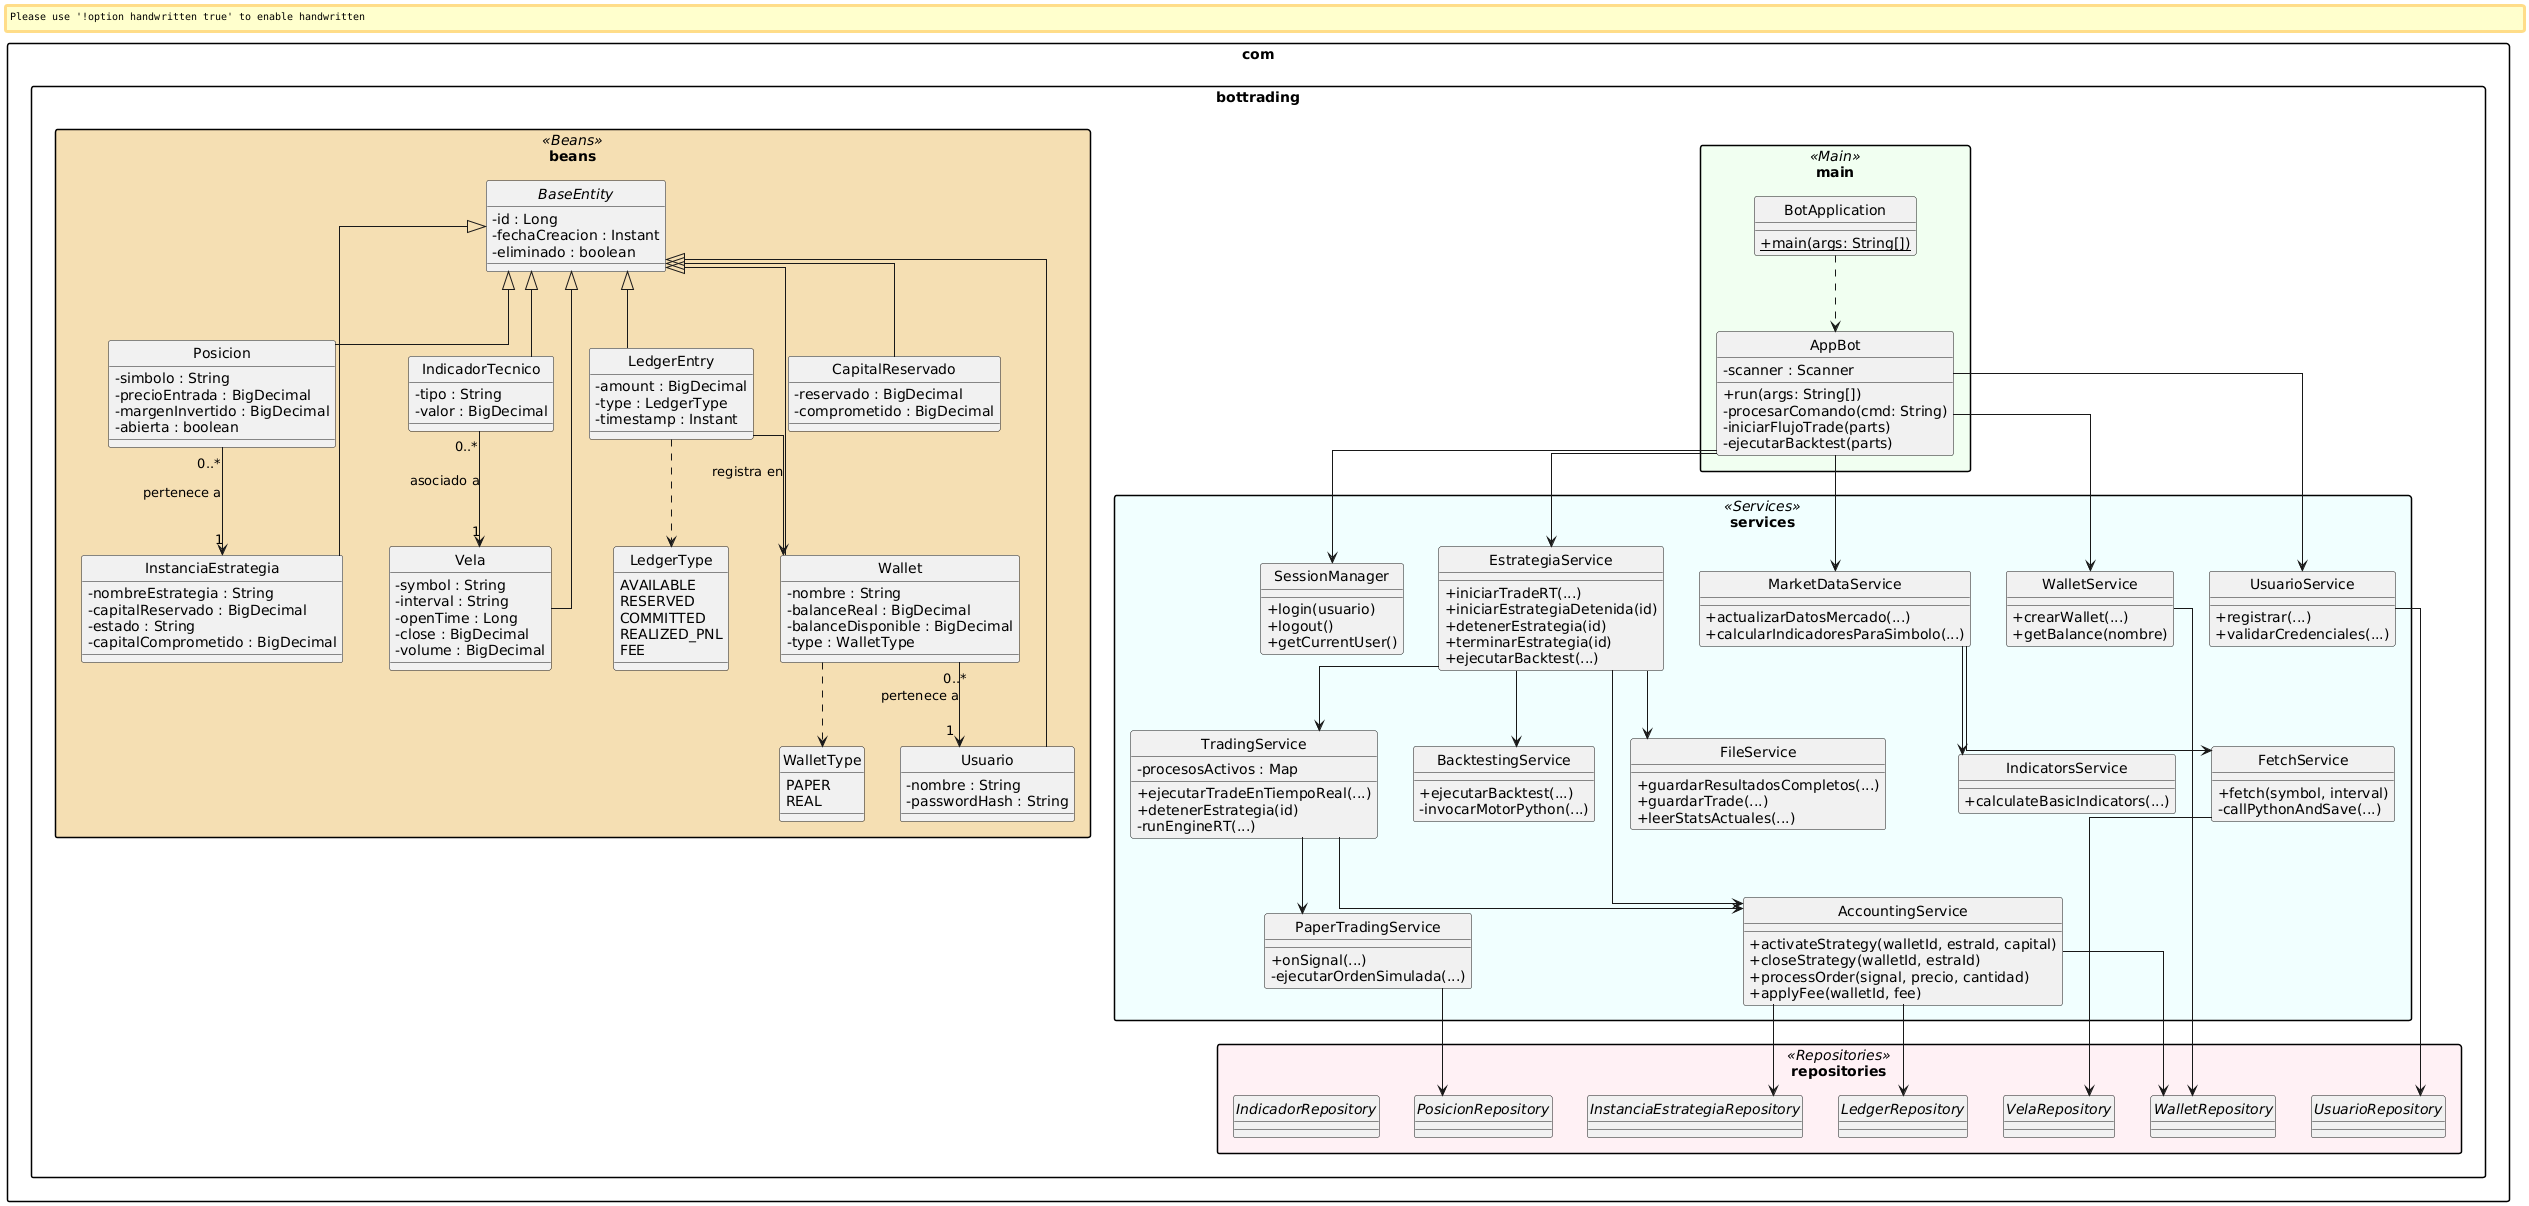
\includegraphics[width=\linewidth]{diagramas-clase/diagrama-clases1.png}
    \caption{Diagrama de clases detallado de la aplicación}
    \label{fig:clases}
\end{figure}

\subsection{Descripción de las Clases del Modelo de Datos}

El diseño del modelo de dominio se basa en entidades JPA que heredan de una clase base común para estandarizar la persistencia. A continuación, se detallan las clases principales que estructuran la lógica de negocio, la gestión de activos y los datos de mercado:
\subsubsection{Modelo de Dominio (Entities)}

\begin{description}
    \item[BaseEntity] Clase abstracta (@MappedSuperclass) que dota a todas las entidades de un identificador único, marca de tiempo de creación y soporte para borrado lógico.
    
    \item[Usuario] Entidad que gestiona la autenticación, almacenando el nombre de usuario y el hash de la contraseña para garantizar la seguridad del acceso.
    
    \item[Wallet] Representa la billetera digital del usuario. Implementa un modelo de doble saldo: \textit{balanceReal} (patrimonio total) y \textit{balanceDisponible} (capital libre para nuevas operaciones). Mantiene una relación \textit{Many-to-One} con la entidad \textit{Usuario}.
    
    \item[WalletType] Enumerado que define la naturaleza de la billetera. Permite distinguir entre \textit{PAPER} (entorno de simulación con dinero ficticio) y \textit{REAL} (conexión con fondos reales en el exchange).
    
    \item[Vela] Entidad fundamental que almacena los datos de mercado en formato OHLCV. Se ha definido una restricción de unicidad compuesta (\textit{UniqueConstraint}) sobre \textit{symbol}, \textit{interval} y \textit{open\_time} para garantizar la integridad de las series temporales utilizadas en el backtesting.
    
    \item[VelaDTO] Objeto de transferencia diseñado para la ingesta masiva de datos. Utiliza tipos \textit{String} para los valores numéricos, evitando la pérdida de precisión decimal durante la deserialización JSON antes de su conversión a \textit{BigDecimal}.

    \item[InstanciaEstrategia] Modela la ejecución de una estrategia de trading. Almacena la configuración de riesgo, el capital asignado, los símbolos a operar y el estado actual de la ejecución (activa, detenida, finalizada).
    
    \item[Posicion] Representa una operación de mercado individual. Está vinculada a una \textit{InstanciaEstrategia} y almacena el precio de entrada, el margen utilizado y el estado de la operación.
    
    \item[LedgerEntry] Registro inmutable de movimientos financieros. Permite auditar el flujo de capital (comisiones, beneficios, reservas) utilizando tipos definidos en \textit{LedgerType}.
    
    \item[CapitalReservado] Entidad auxiliar para gestionar el bloqueo de fondos por estrategia, diferenciando entre capital reservado, comprometido en órdenes activas y riesgo latente.
    
    \item[IndicadorTecnico] Almacena los valores de análisis técnico (ej. RSI, MACD) asociados a un momento de mercado, permitiendo la trazabilidad de las decisiones del algoritmo.
    
    \item[DTOs Auxiliares] (SignalDTO, IndicadorTecnicoDTO) Objetos planos utilizados para la transferencia de datos entre el motor de análisis y la capa de persistencia, desacoplando la lógica de cálculo del almacenamiento.
\end{description}

\subsection{Capa de Acceso a Datos (Repositories)}

La interacción con la base de datos se abstrae mediante el patrón \textit{Repository}, implementado a través de \textbf{Spring Data JPA}. Cada interfaz extiende de \texttt{JpaRepository}, lo que proporciona operaciones CRUD estándar, además de definir consultas personalizadas mediante \textit{Query Methods} y JPQL (Java Persistence Query Language).

A continuación, se describen los repositorios clave y sus responsabilidades específicas:

\begin{description}
    \item[InstanciaEstrategiaRepository] Gestiona la persistencia de las estrategias. Destaca el método \texttt{sumCapitalActivoByWallet}, que realiza una agregación (SUM) para calcular cuánto capital de una billetera está comprometido en estrategias activas, evitando sobregiros. Además, implementa un bloqueo pesimista (\texttt{PESSIMISTIC\_WRITE}) en \texttt{findByIdWithLock} para prevenir condiciones de carrera cuando múltiples hilos intentan modificar el estado de una estrategia simultáneamente.

    \item[VelaRepository] Optimizado para el manejo de series temporales de datos de mercado. Incluye consultas nativas eficientes para obtener la última vela registrada (\texttt{findMaxOpenTime...}), lo cual es crítico para la funcionalidad de descarga incremental de datos (Fetch) sin duplicados. También permite la recuperación ordenada de velas para alimentar los motores de backtesting.

    \item[WalletRepository] Crítico para la integridad financiera. Utiliza bloqueos pesimistas en las operaciones de lectura (\texttt{findByIdWithLock}) para asegurar que ninguna otra transacción modifique el saldo de una billetera mientras se está procesando una orden. Permite consultas filtradas por usuario y tipo de billetera (PAPER/REAL).

    \item[LedgerRepository] Proporciona la trazabilidad contable del sistema. Permite consultar el historial de transacciones ordenado cronológicamente (\texttt{OrderByTimestampDesc}), ya sea filtrando por billetera o por una estrategia específica, facilitando la auditoría de pérdidas y ganancias (PnL).

    \item[PosicionRepository] Gestiona el estado de las operaciones de mercado. Su método \texttt{findByInstanciaAndSimboloAndAbiertaTrue} es fundamental para el motor de trading, ya que permite verificar rápidamente si una estrategia ya tiene una posición abierta en un par de monedas antes de emitir una nueva orden de entrada.

    \item[UsuarioRepository] Encargado de la gestión de identidades. Abstrae las consultas de autenticación y verificación de existencia de usuarios, asegurando que no se registren nombres duplicados (\texttt{existsByNombre}).

    \item[IndicadorRepository] Permite el almacenamiento y recuperación de análisis técnico calculado previamente. Facilita la limpieza de datos obsoletos mediante operaciones transaccionales de borrado masivo (\texttt{deleteByVela}).
\end{description}

\subsection{Capa de Servicio (Business Logic Layer)}

La lógica de negocio de la aplicación se encapsula en servicios de Spring (@Service), los cuales orquestan las operaciones entre los controladores, los repositorios y los motores de cálculo externos. A continuación, se detallan los servicios principales:

\subsubsection{Servicios de Trading y Ejecución}
Estos componentes constituyen el núcleo operativo del sistema, gestionando el ciclo de vida de las estrategias y la comunicación con los procesos de Python.

\begin{description}
    \item[EstrategiaService] Actúa como el orquestador principal del ciclo de vida de las estrategias. Gestiona los comandos de usuario para iniciar (\texttt{iniciarTradeRT}), pausar (\texttt{detenerEstrategia}) y liquidar (\texttt{terminarEstrategia}) las instancias. Coordina la reserva de capital con \textit{AccountingService} antes de delegar la ejecución técnica al \textit{TradingService}.

    \item[TradingService] Servicio de bajo nivel encargado de la gestión de hilos y procesos del sistema operativo. Utiliza un \texttt{ExecutorService} para lanzar y supervisar los scripts de Python (\texttt{engine\_rt.py}) en hilos independientes. Implementa un mapa concurrente (\texttt{ConcurrentHashMap}) para mantener el control de los procesos activos y permitir su detención forzosa en caso de emergencia.

    \item[PaperTradingService] Simula la ejecución de órdenes en un entorno controlado. Recibe las señales de compra/venta (SignalDTO) desde el motor de Python, valida las reglas de gestión de riesgo y, si procede, registra las posiciones simuladas en la base de datos, comunicando los resultados financieros al servicio de contabilidad.

    \item[BacktestingService] Facilita la validación histórica de estrategias. Prepara los datos de velas almacenados en la base de datos, los transforma a formato JSON y los envía al motor de backtesting (\texttt{engine\_backtest.py}). Posteriormente, captura los resultados y estadísticas para su almacenamiento.
\end{description}

\subsubsection{Servicios de Gestión de Datos y Contabilidad}
Garantizan la integridad de la información financiera y la disponibilidad de datos de mercado.

\begin{description}
    \item[AccountingService] Servicio transaccional crítico (`@Transactional`) que gestiona el libro mayor (\textit{Ledger}). Es responsable de todas las operaciones monetarias: reservar fondos al activar una estrategia (`activateStrategy`), mover capital a margen comprometido (`commitCapital`) y liquidar beneficios o pérdidas (`closeTrade`). Implementa bloqueos pesimistas en las billeteras para evitar condiciones de carrera en el saldo.

    \item[FetchService] Implementa la lógica de sincronización de datos de mercado (ETL). Utiliza un algoritmo de descarga incremental: verifica la última vela registrada en la base de datos y solicita a la API externa únicamente los datos nuevos, optimizando el ancho de banda y el tiempo de procesamiento.

    \item[MarketDataService] Actúa como una fachada (\textit{Facade}) que simplifica la interacción con los datos de mercado. Coordina la descarga de velas a través de \textit{FetchService} y el cálculo posterior de indicadores técnicos mediante \textit{IndicatorsService}, asegurando que los datos estén actualizados antes de cualquier análisis.
\end{description}

\subsubsection{Servicios de Infraestructura y Usuarios}
Proporcionan funcionalidades transversales de soporte al sistema.

\begin{description}
    \item[UsuarioService] Gestiona el ciclo de vida de los usuarios. Implementa el registro con hash de contraseñas (utilizando \textit{HashUtils}) y la validación de credenciales. Además, soporta el borrado lógico de cuentas para mantener la integridad referencial de los datos históricos.

    \item[FileService] Encargado de la persistencia en el sistema de archivos. Genera y actualiza los reportes CSV de operaciones (\textit{trades}) y estadísticas acumuladas (\textit{stats}). Incluye mecanismos de bloqueo para evitar corrupción de archivos durante la escritura concurrente.
\end{description}

\subsection{Capa de Aplicación y Utilidades Transversales}

Para complementar la lógica de negocio, se han implementado componentes de infraestructura que gestionan el ciclo de vida de la aplicación, la interacción con el usuario y la seguridad.

\subsubsection{Punto de Entrada y Configuración (Main)}
La clase \texttt{BotApplication} es el punto de entrada de la aplicación Spring Boot. Implementa una carga personalizada de variables de entorno (utilizando la librería \textit{Dotenv}) para configurar la conexión a base de datos de forma segura sin hardcodear credenciales. Además, silencia los logs internos de Spring y Hibernate para ofrecer una interfaz de línea de comandos (CLI) limpia al usuario.

\subsubsection{Interfaz de Usuario (CLI)}
La interacción se gestiona mediante la clase \texttt{AppBot}, que implementa la interfaz \texttt{CommandLineRunner}. Actúa como un bucle de eventos que lee los comandos del usuario (ej: \textit{trade}, \textit{fetch}, \textit{backtest}) y delega la ejecución al servicio correspondiente. Incluye validaciones de sesión mediante \texttt{SessionManager} antes de permitir operaciones críticas.

\subsubsection{Gestión de Sesión y Seguridad}
\begin{description}
    \item[SessionManager] Componente con ámbito de Singleton que mantiene en memoria el estado del usuario actual (\texttt{currentUser}). Facilita el acceso global al contexto de seguridad y asegura que, al detener la aplicación (\texttt{@PreDestroy}), se cierren ordenadamente todas las estrategias activas.
    
    \item[HashUtils] Clase de utilidad estática que encapsula la criptografía de contraseñas utilizando \textbf{BCrypt}. Garantiza que las credenciales de los usuarios se almacenen de forma segura (hasheadas) y nunca en texto plano, cumpliendo con los estándares de seguridad básicos.
\end{description}

\subsubsection{Utilidades del Sistema}
\begin{description}
    \item[PathConfig] Centraliza la gestión de rutas del sistema de archivos. Resuelve dinámicamente la ubicación de los scripts de Python (\textit{engine\_rt.py}, \textit{fetcher.py}) y las carpetas de resultados, independientemente de desde dónde se ejecute el JAR, evitando errores de "archivo no encontrado" en despliegues.
    
    \item[AppConstants] Define el protocolo de comunicación entre Java y Python. Contiene las claves de los objetos JSON (ej: \texttt{KEY\_SYMBOL}, \texttt{KEY\_PRICE}) y las cabeceras de los archivos CSV, asegurando que ambos lenguajes hablen el mismo "idioma" sin errores de tipado.
    
    \item[ConsoleLoader] Mejora la experiencia de usuario (UX) mostrando animaciones de carga (spinners o puntos) en la consola durante operaciones largas como la descarga de datos o el entrenamiento de modelos, proporcionando feedback visual de que el sistema sigue procesando.
\end{description}

\subsubsection{Servicios de Gestión de Datos y Contabilidad}
Garantizan la integridad de la información financiera y la disponibilidad de datos de mercado.

\begin{description}
    \item[AccountingService] Servicio transaccional crítico (`@Transactional`) que gestiona el libro mayor (\textit{Ledger}). Es responsable de todas las operaciones monetarias: reservar fondos al activar una estrategia (`activateStrategy`), mover capital a margen comprometido (`commitCapital`) y liquidar beneficios o pérdidas (`closeTrade`). Implementa bloqueos pesimistas en las billeteras para evitar condiciones de carrera en el saldo.

    \item[FetchService] Implementa la lógica de sincronización de datos de mercado (ETL). Utiliza un algoritmo de descarga incremental: verifica la última vela registrada en la base de datos y solicita a la API externa únicamente los datos nuevos, optimizando el ancho de banda y el tiempo de procesamiento.

    \item[MarketDataService] Actúa como una fachada (\textit{Facade}) que simplifica la interacción con los datos de mercado. Coordina la descarga de velas a través de \textit{FetchService} y el cálculo posterior de indicadores técnicos mediante \textit{IndicatorsService}, asegurando que los datos estén actualizados antes de cualquier análisis.
\end{description}

\subsubsection{Servicios de Infraestructura y Usuarios}
Proporcionan funcionalidades transversales de soporte al sistema.

\begin{description}
    \item[UsuarioService] Gestiona el ciclo de vida de los usuarios. Implementa el registro con hash de contraseñas (utilizando \textit{HashUtils}) y la validación de credenciales. Además, soporta el borrado lógico de cuentas para mantener la integridad referencial de los datos históricos.

    \item[FileService] Encargado de la persistencia en el sistema de archivos. Genera y actualiza los reportes CSV de operaciones (\textit{trades}) y estadísticas acumuladas (\textit{stats}). Incluye mecanismos de bloqueo para evitar corrupción de archivos durante la escritura concurrente.
\end{description}

\subsection{Capa de Aplicación y Utilidades Transversales}

Para complementar la lógica de negocio, se han implementado componentes de infraestructura que gestionan el ciclo de vida de la aplicación, la interacción con el usuario y la seguridad.

\subsubsection{Punto de Entrada y Configuración (Main)}
La clase \texttt{BotApplication} es el punto de entrada de la aplicación Spring Boot. Implementa una carga personalizada de variables de entorno (utilizando la librería \textit{Dotenv}) para configurar la conexión a base de datos de forma segura sin hardcodear credenciales. Además, silencia los logs internos de Spring y Hibernate para ofrecer una interfaz de línea de comandos (CLI) limpia al usuario.

\subsubsection{Interfaz de Usuario (CLI)}
La interacción se gestiona mediante la clase \texttt{AppBot}, que implementa la interfaz \texttt{CommandLineRunner}. Actúa como un bucle de eventos que lee los comandos del usuario (ej: \textit{trade}, \textit{fetch}, \textit{backtest}) y delega la ejecución al servicio correspondiente. Incluye validaciones de sesión mediante \texttt{SessionManager} antes de permitir operaciones críticas.

\subsubsection{Gestión de Sesión y Seguridad}
\begin{description}
    \item[SessionManager] Componente con ámbito de Singleton que mantiene en memoria el estado del usuario actual (\texttt{currentUser}). Facilita el acceso global al contexto de seguridad y asegura que, al detener la aplicación (\texttt{@PreDestroy}), se cierren ordenadamente todas las estrategias activas.
    
    \item[HashUtils] Clase de utilidad estática que encapsula la criptografía de contraseñas utilizando \textbf{BCrypt}. Garantiza que las credenciales de los usuarios se almacenen de forma segura (hasheadas) y nunca en texto plano, cumpliendo con los estándares de seguridad básicos.
\end{description}

\subsubsection{Utilidades del Sistema}
\begin{description}
    \item[PathConfig] Centraliza la gestión de rutas del sistema de archivos. Resuelve dinámicamente la ubicación de los scripts de Python (\textit{engine\_rt.py}, \textit{fetcher.py}) y las carpetas de resultados, independientemente de desde dónde se ejecute el JAR, evitando errores de "archivo no encontrado" en despliegues.
    
    \item[AppConstants] Define el protocolo de comunicación entre Java y Python. Contiene las claves de los objetos JSON (ej: \texttt{KEY\_SYMBOL}, \texttt{KEY\_PRICE}) y las cabeceras de los archivos CSV, asegurando que ambos lenguajes hablen el mismo "idioma" sin errores de tipado.
    
    \item[ConsoleLoader] Mejora la experiencia de usuario (UX) mostrando animaciones de carga (spinners o puntos) en la consola durante operaciones largas como la descarga de datos o el entrenamiento de modelos, proporcionando feedback visual de que el sistema sigue procesando.
\end{description}

\subsection{Diagramas de Flujo}
A continuación, se describen los procesos principales del sistema, desde la autenticación hasta la ejecución de estrategias en tiempo real.

\subsubsection{Gestión de Usuarios y Acceso}
El flujo de entrada al sistema valida las credenciales y gestiona la sesión del usuario, permitiendo también el acceso a la ayuda del sistema (ver Figura \ref{fig:login}).

\begin{figure}[h!]
    \centering
    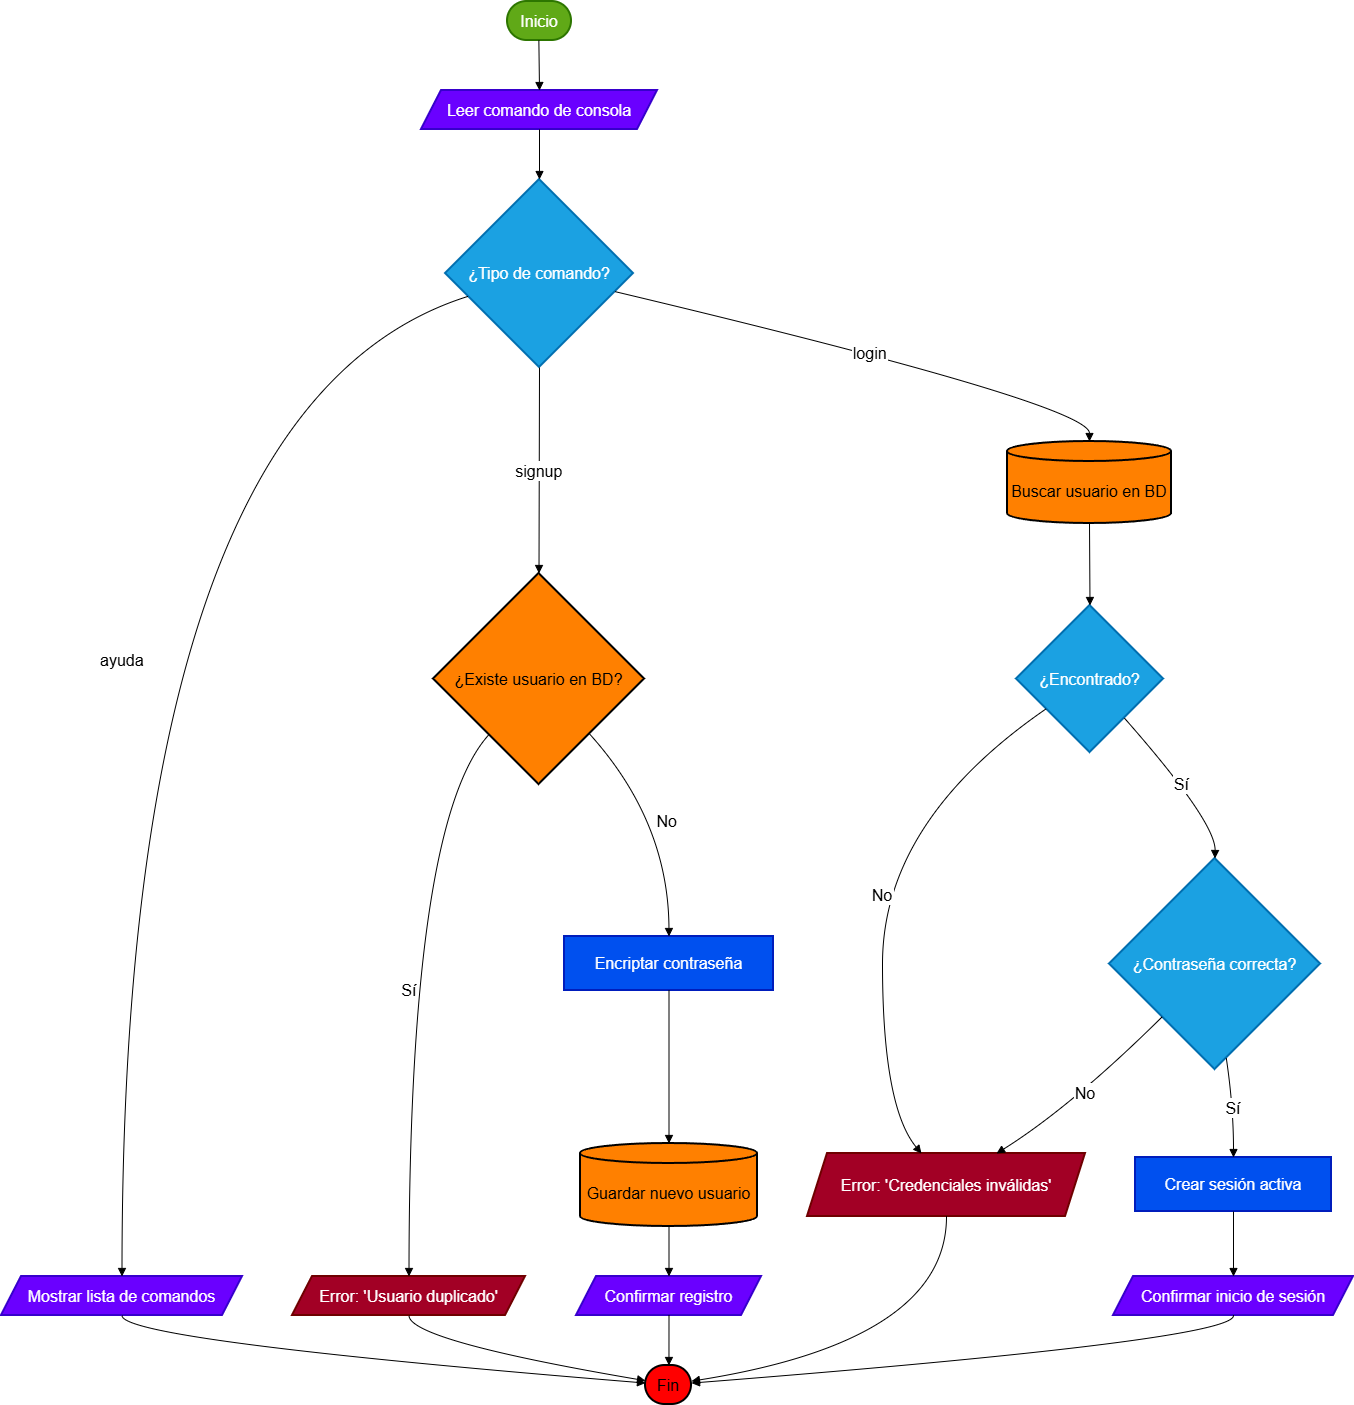
\includegraphics[width=0.9\linewidth]{diagramas-flujo/inicio-registro-ayuda.png}
    \caption{Flujo de autenticación (Login/Signup) y Ayuda}
    \label{fig:login}
\end{figure}

\subsubsection{Gestión de Capital (Wallets)}
La creación y consulta de billeteras virtuales (Paper Trading) se valida contra la sesión actual del usuario, asegurando la integridad de los datos financieros simulados.

\begin{figure}[h!]
    \centering
    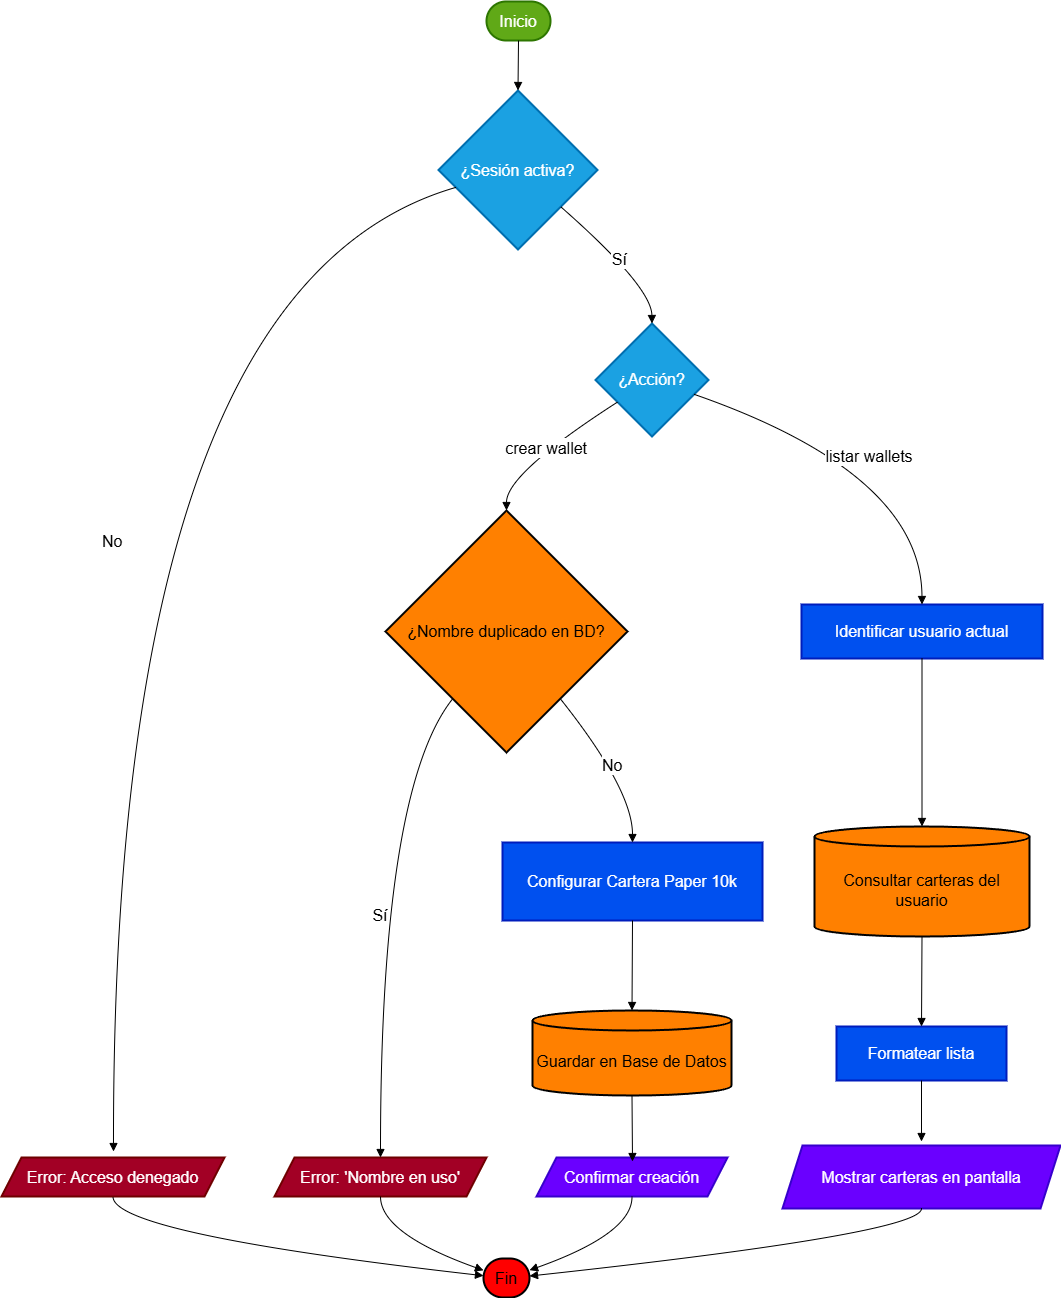
\includegraphics[width=0.9\linewidth]{diagramas-flujo/creacion-listado-wallets.png}
    \caption{Proceso de creación y listado de Wallets}
    \label{fig:wallets}
\end{figure}

\subsubsection{Obtención de Datos (ETL)}
El sistema implementa un mecanismo de descarga incremental para optimizar las peticiones a la API de Binance, tal y como se ilustra en la Figura \ref{fig:fetch}.



\begin{figure}[H]
    \centering
    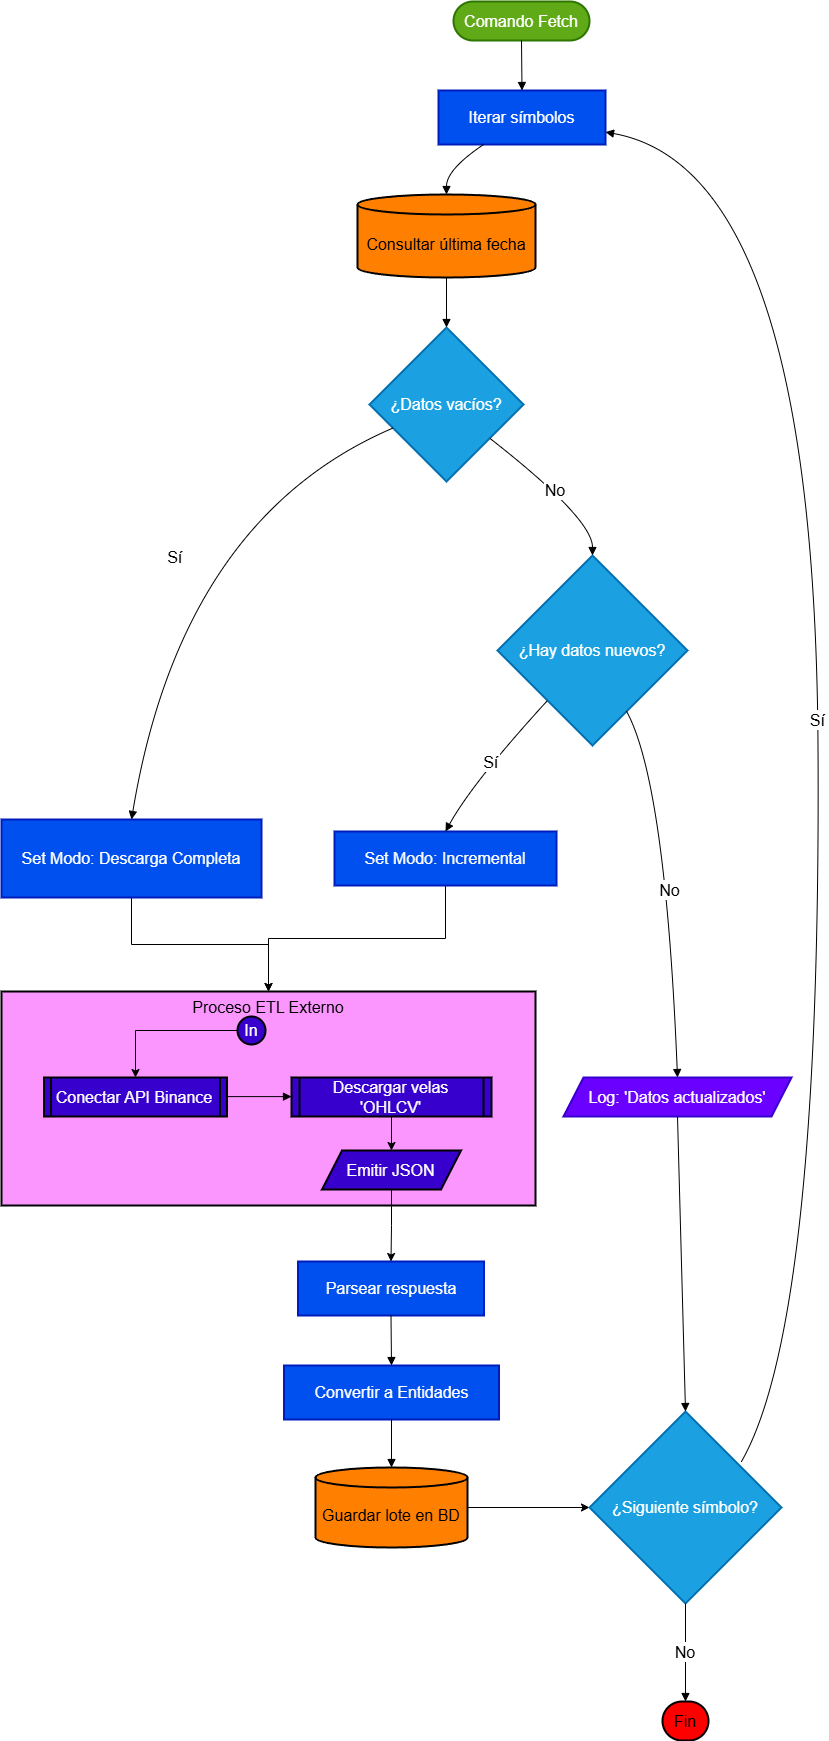
\includegraphics[width=0.65\linewidth]{diagramas-flujo/fetch.png}
    \caption{Flujo de obtención y sincronización de datos de mercado (Fetch)}
    \label{fig:fetch}
\end{figure}

\subsubsection{Gestión de Estrategias}
El ciclo de vida de las estrategias permite al usuario listar los scripts disponibles en disco y consultar el estado de las instancias en base de datos.

\begin{figure}[H]
    \centering
    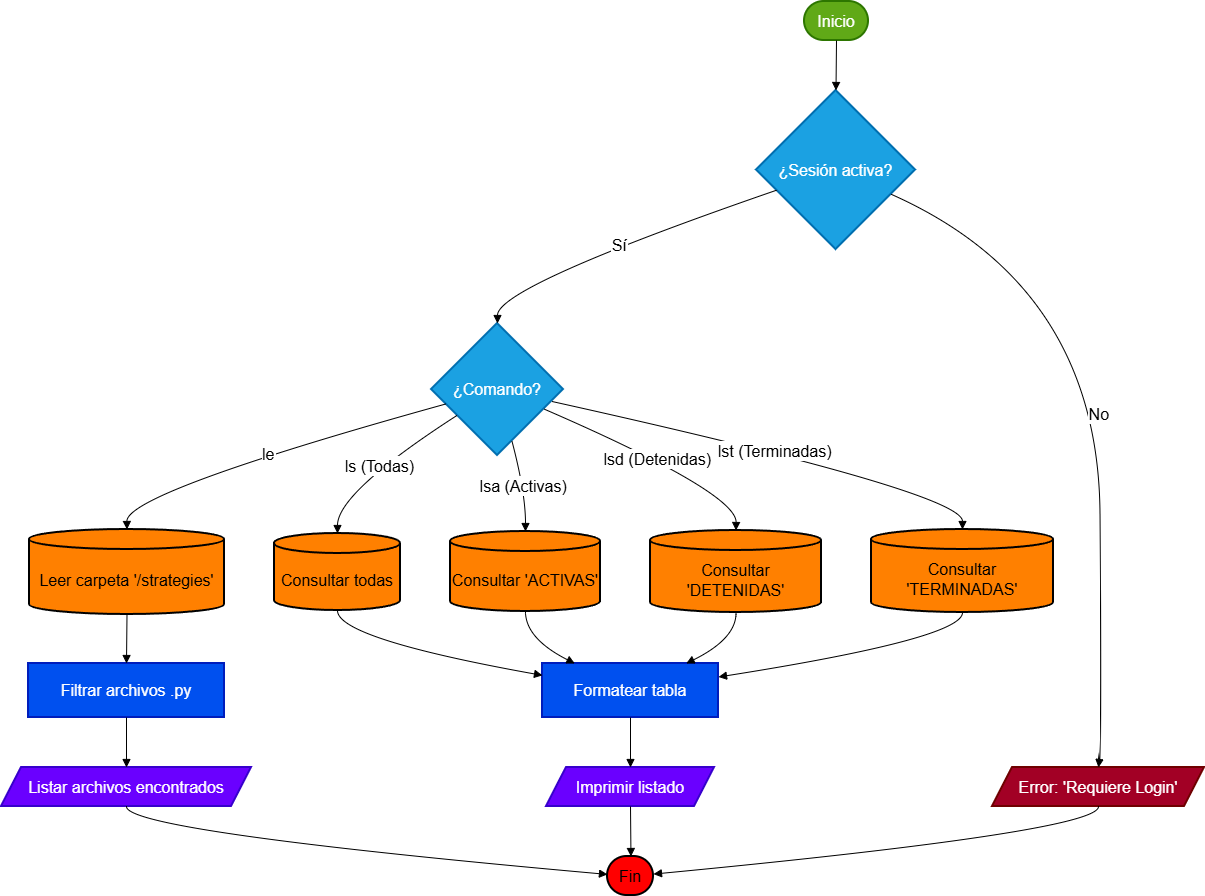
\includegraphics[width=0.9\linewidth]{diagramas-flujo/listado-estrategias.png}
    \caption{Flujo de comandos de listado (ls, le, lsa)}
    \label{fig:listado}
\end{figure}

La Figura \ref{fig:gestion} detalla las operaciones de control de ciclo de vida: pausar (\textit{stop}), reanudar (\textit{start}) y liquidar (\textit{term}) una estrategia.

\begin{figure}[H]
    \centering
    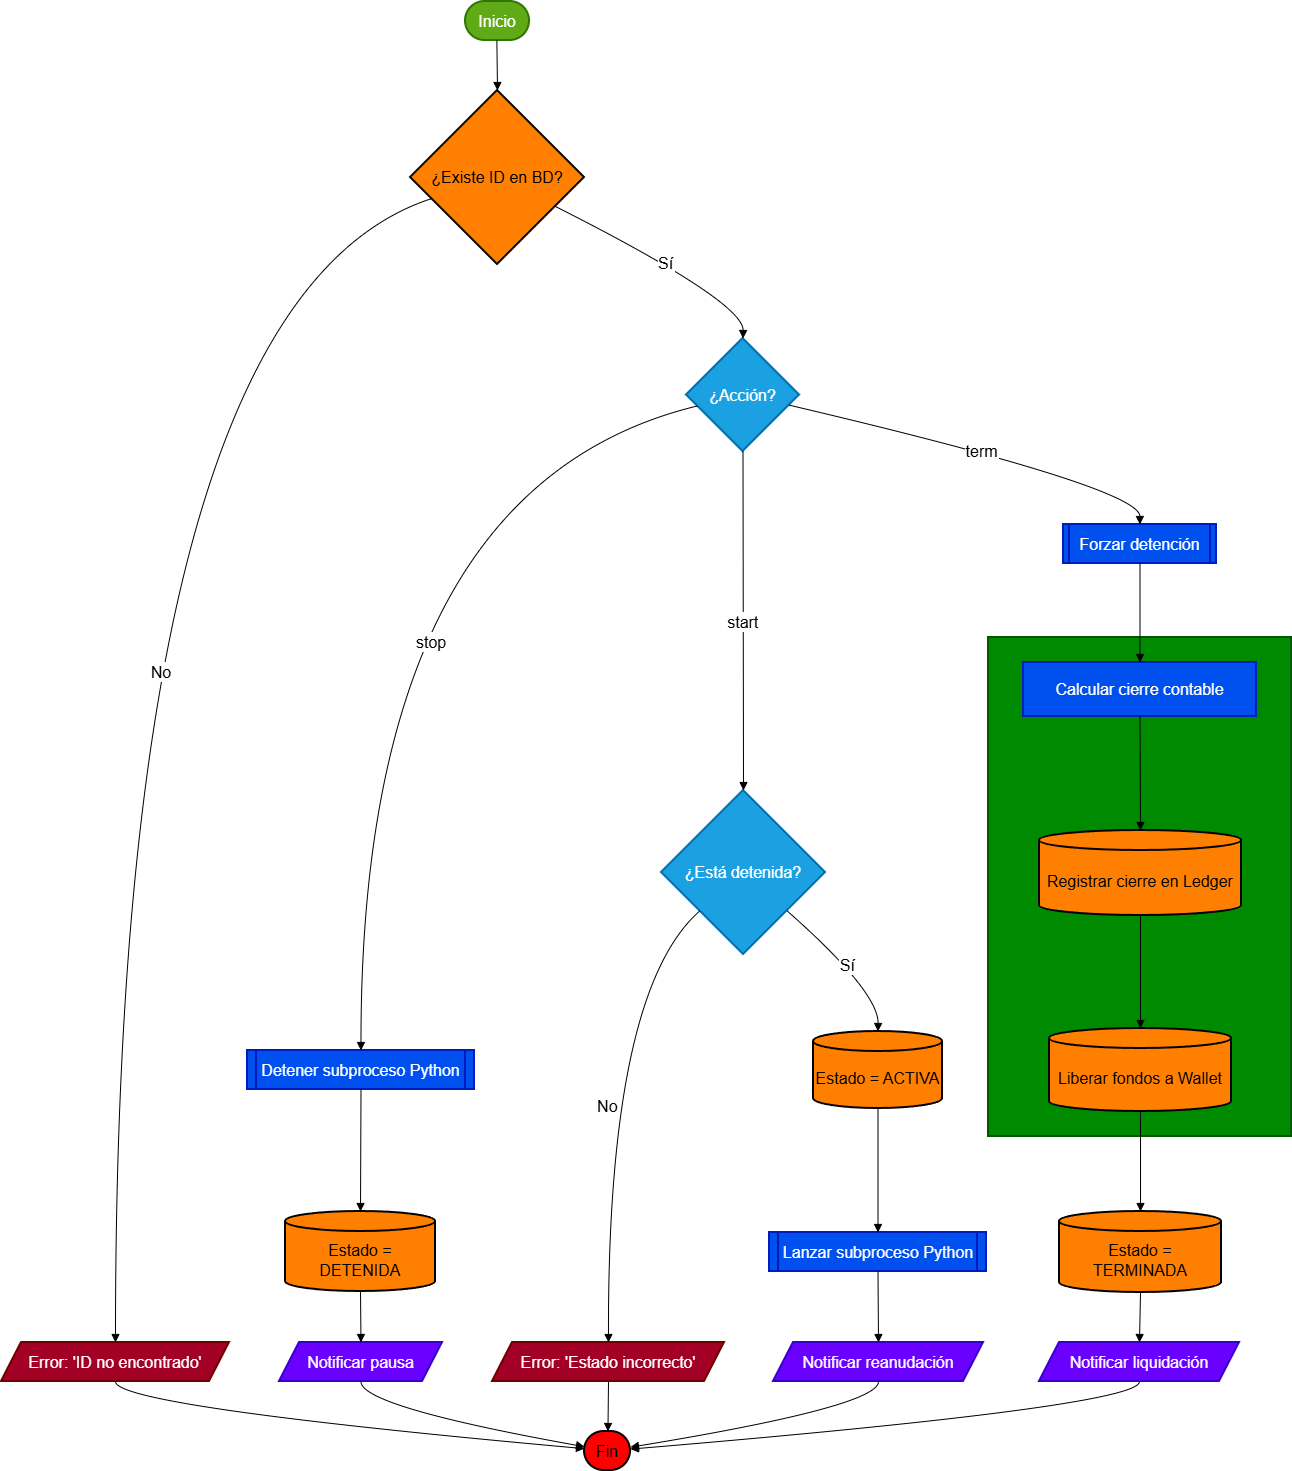
\includegraphics[width=0.9\linewidth]{diagramas-flujo/gestion-estrategias.png}
    \caption{Ciclo de vida: Start, Stop y Terminate}
    \label{fig:gestion}
\end{figure}

\subsubsection{Motores de Ejecución}
El núcleo del sistema reside en los motores de simulación y ejecución real. La Figura \ref{fig:backtest} muestra el flujo de validación histórica.

\begin{figure}[H]
    \centering
    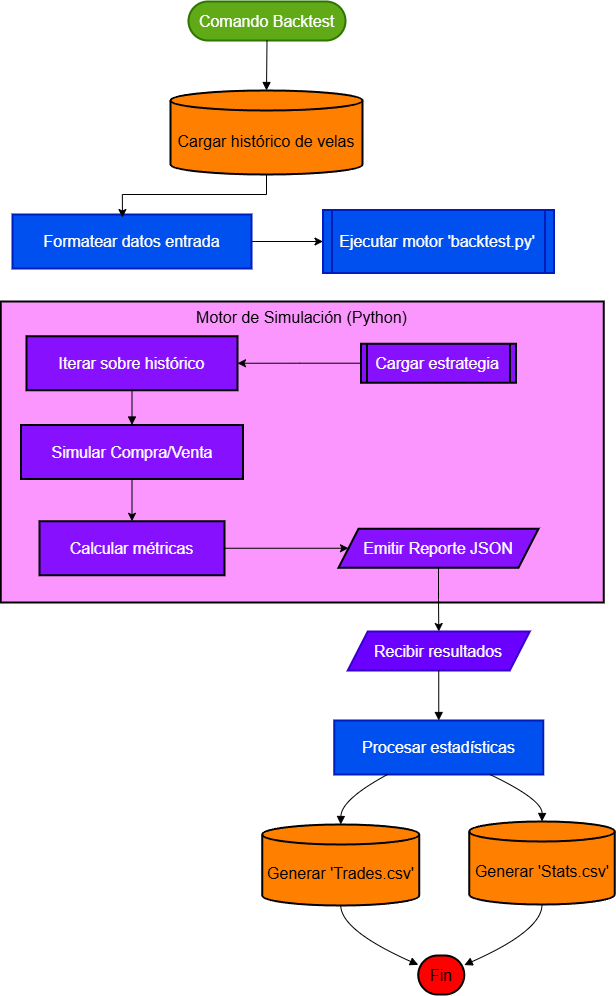
\includegraphics[width=0.8\linewidth]{diagramas-flujo/backtest.png}
    \caption{Flujo de ejecución del motor de Backtesting}
    \label{fig:backtest}
\end{figure}

Finalmente, la Figura \ref{fig:trade} ilustra la arquitectura híbrida Java-Python para la operativa en tiempo real, incluyendo la gestión transaccional del Ledger.

\begin{figure}[H]
    \centering
    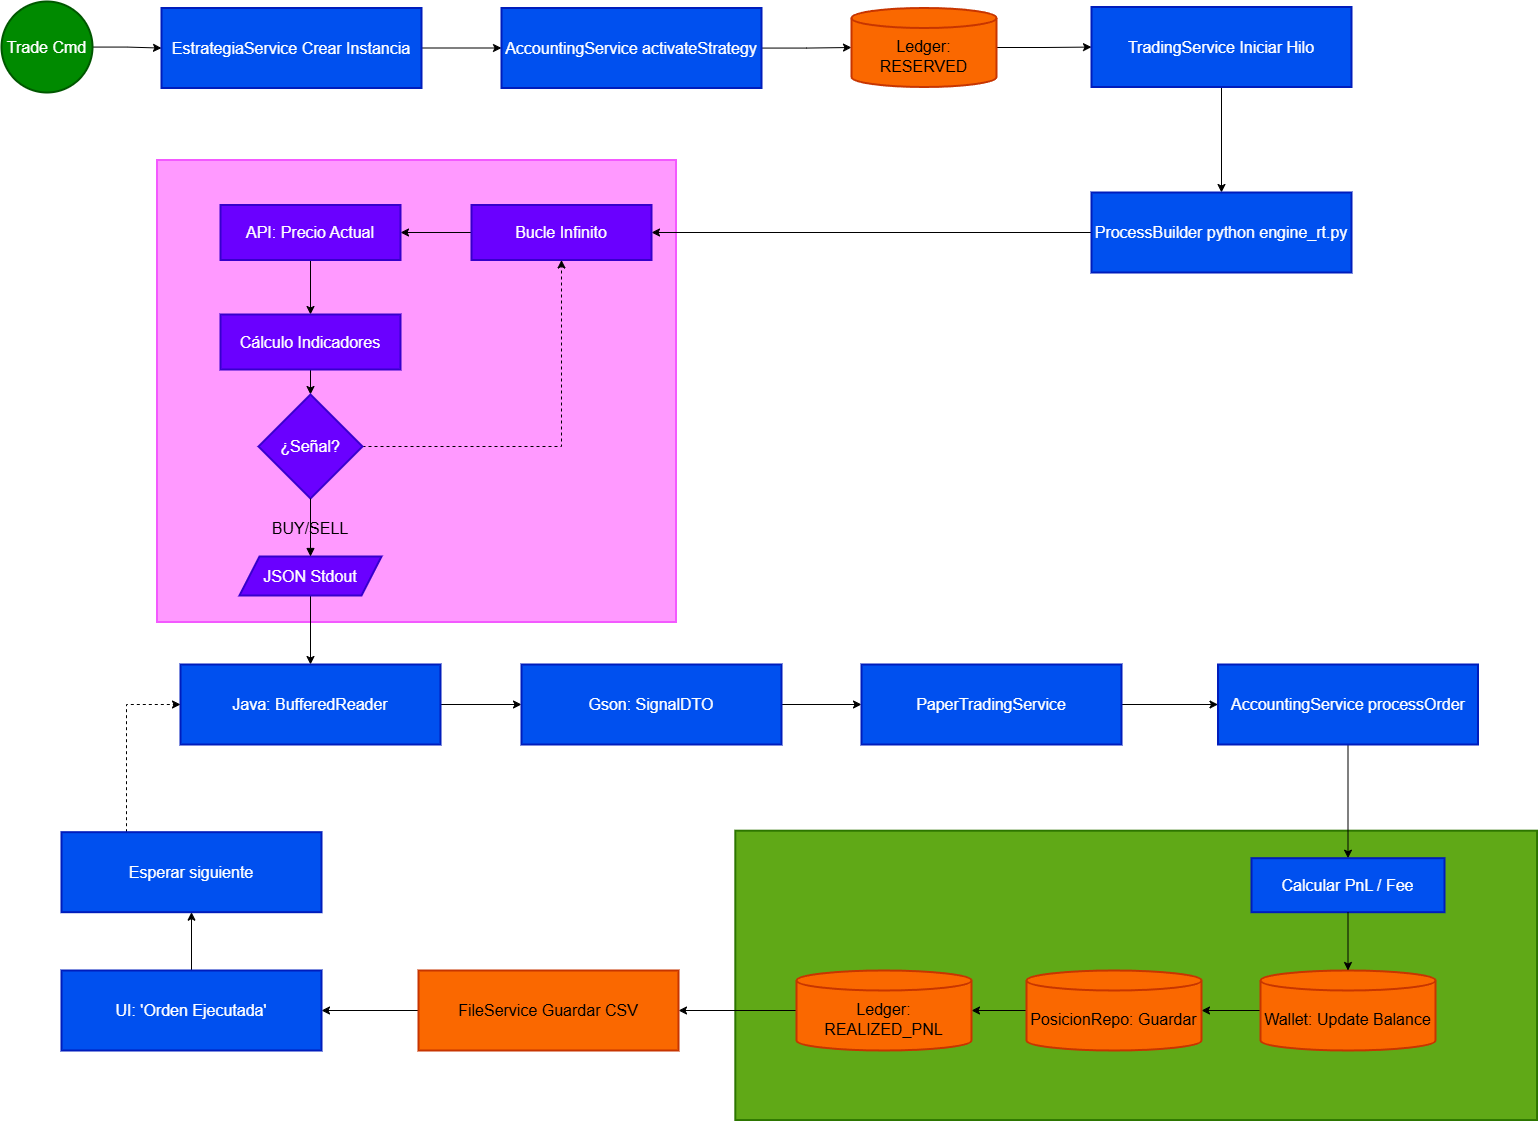
\includegraphics[width=\linewidth]{diagramas-flujo/trade.png}
    \caption{Flujo de Trading en Tiempo Real y comunicación Java-Python}
    \label{fig:trade}
\end{figure}

\subsection{Glosario}

Para la correcta comprensión del dominio del problema, se definen a continuación los conceptos económicos y técnicos fundamentales utilizados en el diseño del sistema:

\begin{description}
    \item[Exchange (Casa de Intercambio)] Plataforma digital que facilita la compraventa de activos financieros, como criptomonedas, actuando como intermediario y proveedor de liquidez y datos de mercado. En este proyecto, se simula la interacción con un Exchange (ej. Binance) para la obtención de datos históricos y precios en tiempo real.

    \item[OHLCV] Acrónimo de \textit{Open, High, Low, Close, Volume}. Es el formato estándar para representar la acción del precio de un activo financiero durante un intervalo de tiempo específico (Vela o \textit{Candlestick}). 
    \begin{itemize}
        \item \textbf{Open:} Precio al inicio del intervalo.
        \item \textbf{High:} Precio máximo alcanzado.
        \item \textbf{Low:} Precio mínimo alcanzado.
        \item \textbf{Close:} Precio al cierre del intervalo.
        \item \textbf{Volume:} Cantidad total del activo negociada.
    \end{itemize}
    En el sistema, esta estructura se modela mediante la entidad \texttt{Vela}.

    \item[Wallet (Billetera Digital)] Entidad encargada de custodiar y gestionar el capital del usuario. En el contexto de la aplicación, se implementa un sistema de \textit{doble saldo} para distinguir entre el patrimonio total (\textit{Balance Real}) y el capital libre para operar (\textit{Balance Disponible}).

    \item[Ledger (Libro Mayor)] Registro contable inmutable y secuencial donde se anotan todas las transacciones financieras. Su función es garantizar la integridad de los datos y permitir la auditoría de movimientos como reservas de fondos, comisiones o beneficios realizados. En el sistema, cada movimiento genera una entrada de tipo \texttt{LedgerEntry}.

    \item[Estrategia de Trading] Conjunto de reglas lógicas y matemáticas que determinan de forma autónoma cuándo comprar o vender un activo. Estas reglas se definen en scripts de Python y son orquestadas por la entidad \texttt{InstanciaEstrategia} en Java.

    \item[Indicador Técnico] Cálculo matemático derivado del precio y/o volumen histórico de un activo, utilizado para predecir movimientos futuros del mercado.
    \begin{itemize}
        \item \textbf{RSI (Relative Strength Index):} Oscilador de momento que mide la velocidad y el cambio de los movimientos de precios para identificar condiciones de sobrecompra o sobreventa.
        \item \textbf{MACD (Moving Average Convergence Divergence):} Indicador de seguimiento de tendencia que muestra la relación entre dos medias móviles del precio de un activo.
    \end{itemize}
    El sistema persiste estos valores en la entidad \texttt{IndicadorTecnico} para su análisis posterior.
    
    \item[Paper Trading] Modalidad de simulación bursátil que permite operar con dinero ficticio en un entorno de mercado real. El sistema soporta este modo mediante el servicio \texttt{PaperTradingService}, permitiendo validar estrategias sin riesgo financiero.

    \item[PnL (Profit and Loss)] Término que hace referencia a las ganancias o pérdidas netas obtenidas en una operación o en un periodo determinado. Se calcula como la diferencia entre el valor de salida y el valor de entrada de una posición, descontando las comisiones.
\end{description}

% --- Referencias ---
\newpage
\printbibliography[heading=bibintoc, title={Referencias Bibliográficas}]

\end{document}